
\section{\name}
\label{sec:method}

In this section, we present our framework for inference-time contextual sparsity search for LLMs.  We introduce the sparsity predictor for MLPs in Section~\ref{sec:routing_mlp} and for attention heads in Section~\ref{sec:routing_attn}. \name{}'s workflow is shown in Figure~\ref{fig:workflow_main}.  Section~\ref{sec:hide_overhead} discusses exploiting our observation on LLMs to avoid the sparse prediction overhead with theoretical guarantees. In Section~\ref{sec:sparse_matmul}, we present our optimized implementation that enables end-to-end latency reduction. More details are presented in Section~\ref{appendix:method}.



% We can formulate LLMs as a NNS problem: for each layer, the model parameters can be regarded as database points in NNS problem. The sparsity predictor can be seen as a NNS data structure. The task of predicting contextual sparsity is basically running query for NNS data structure. However, there are types of queries in our LLMs situations. The first type query is, we treat the output from previous layer as a query point in NNS data structure directly. The second type query is we treat the output from a few layers before (instead of exact previous layer). %regarding output from previous layer or input to the current layer 
% %as a query point in NNS data structure.
% The next key observation is called ``slowly change''. Such phenomenon comes from the following scenario. The  scenario is that the output from two ``close'' enough layers, are similar. 

% Intuitively, Due to those slowly change property. Every time when we run query, it is not necessary to always use type 1 query. Using type 2 query can potentially speedup the inference stage, and in the meanwhile maintain accuracy.

\subsection{Contextual Sparsity Prediction in MLP Blocks}
\label{sec:routing_mlp}
As explained in Section~\ref{sec:obs_computation}, MLP blocks are one of the major bottlenecks for the LLM generation ($\frac{2}{3}$ of the FLOPs and IOs). In this section, we discuss how we achieve wall-clock time speed-up with contextual sparsity in the MLP blocks.

\textbf{Challenge} Figure~\ref{obs:175b-sparsity-mlp} shows that for a given token, the contextual sparsity of 95\% is possible.  The contextual sparsity in the MLP block can be identified after computing the activation. However, this only demonstrates the existence of contextual sparsity but brings no benefits in terms of efficiency. A fast and precise prediction is needed to exploit contextual sparsity for end-to-end efficiency. The naive way is to select a subset of neurons randomly. Unsurprisingly, random selection fails to identify the accurate contextual sparsity, resulting in drastic model degradation. 

\textbf{A Near-Neighbor Search Problem:}  Recall that we verify the existence of contextual sparsity by recording which neurons yield significant norms. Essentially, given the input, the goal is to search for the neurons that have high inner products with the input, because the activation function ``filters" low activation. Thus, we formulate the contextual sparsity prediction of an MLP layer as the classical near-neighbor search problem under the inner product metric. 
\begin{definition}[Approximate $\maxip$ in MLP]\label{def:approximate_maxip:informal}
Let $c \in (0,1)$ and $\tau \in (0,1)$ denote two parameters.
Given an $n$-vector dataset $W^1 \subset \mathbb{S}^{d-1}$ on a unit sphere, the objective of the $(c,\tau)$-{$\maxip$} is to construct a data structure that, given a query $y \in \mathbb{S}^{d-1}$ such that $\max_{w\in W^1}\langle y, w \rangle \geq \tau$, it retrieves a vector $z$ from $W^1$ that satisfies $\langle y, z \rangle \geq c \cdot \max_{w \in W^1} \langle y,w \rangle$.
\end{definition}

% \iffalse
\begin{remark}
Our $W^1$ (first linear layer) and $y$ (input embedding) in MLP blocks can be viewed as the dataset and query  in Definition~\ref{def:approximate_maxip:informal}  respectively.
\end{remark}
% \fi

%Let the input $y$ be the query and $W^1$ be the data in NNS. 

% Let $X \in \R^{d}$ denote the input to Expand-MLP, $w \in \R^{ d \times 4d}$ denote the weights of Expand-MLP and each column $w_i \in \R^{d}$ ($i \in [4d]$) corresponds to the weight of the $i$-th neuron.  $w_i, i \in [4d]$ is considered the data $x\in \R^{d}$ is considered as a query. Near-neighbor search methods can be adopted to search for a set $S^M_x$ of $w_i$ that are close to $x$ under the inner product metric. 

\textbf{Design} The standard state-of-the-art near-neighbor search methods and implementations slow down the computation. Take OPT-175B where $d$ is 12288 as an example. HNSW~\cite{malkov2018efficient} requires more than 10ms, and FAISS~\cite{johnson2019billion} requires more than 4ms, while the MLP computation is only 0.2ms. The high dimensionality and complications of data structure implementation on GPU make the search time longer than the MLP computation. Therefore, we choose a neural network classifier as our near-neighbor search method to exploit the fast matrix multiplication on GPU. For each MLP block, we train a small two-layer fully connected network to predict contextual sparsity. Collecting training data is straightforward because we know the contextual sparsity using dense computation. The training algorithm is summarized in Algorithm~\ref{alg:sparse_predictor_training}. The sparsified computation in $W^1$ has two steps: (1) Given $y$, the sparsity predictor $\mathsf{SP}_{M}$ predicts a set $S_M$ of important neurons in weights $W^1$. (2) Compute the sparsified MLP defined in Eq.~\eqref{eq:MLP_S_y}. Note here the sparsity in MLP is highly structured.
% by multiplying $y$ with $i \in S$. Computation at the Expand-MLP is sparse multiplication because the weights are sparsified. This results in sparse activations, which naturally sparsify the Contract-MLP computation.

 % We collect training data for every transformer layer and train the classifier at each transformer layer using binary cross-entropy loss. 



% \textbf{Importance Signal}
% The activation function after the Expand-MLP will zeros out small outputs. Thus, we use the magnitude of the inner product between $x$ with $w_i$ as the importance score of each neuron. This can be formulated as a standard near-neighbor search problem. $w_i, i \in [4d]$ is considered as the data, and for a query $x$, the MLP sparse predictor $\mathsf{SP}^M$would like to identify a set $S^w$ of $w_i$ that is close to $x$ under inner product metric. 



% In this section, we describe a simple learning algorithm to learn a neural network classifier as our neighbor search method.  

% Given the high dimensionality of activation and A100 characteristics, we design a neural network classifier to reduce query overhead.
% We view every neuron $w_i$ in Expand-MLP as a class. For a token $q \in \R^{d}$, we label the activated neuron as positive and the rest as negative. We collect training data for every transformer layer and train the classifier at each transformer layer using binary cross-entropy loss. 

% The following code describes the architecture of our classifier. Because $h \ll d$, the latency of such a classifier is significantly less than Expand-MLP on the same hardware.

% \begin{lstlisting}[language=Python]
% predictor = torch.nn.Sequential(
%     torch.nn.Linear(d, h, bias=None),
%     torch.nn.Linear(h, 4d, bias=None))
% \end{lstlisting}

% As we discussed in Section 1, we observe high sparsity after Expand MLP. For example, in OPT175b, less than 5\% of neurons are activated after the activation function. Near neigobor search methods can be adopted here to reduce the computation at Expand-MLP. 

\begin{algorithm}
   \caption{Sparse Predictor Training}
   \label{alg:sparse_predictor_training}
\begin{algorithmic}
 \State \textbf{Input}: A pre-trained LLM block with parameter set $M$, token embedding set at block $M = \{ x_i \}_{i\in [N]}$, threshold $t$
\State \textbf{Sparse Predictor} ${\cal SP}$
 % \State \textbf{Sparse Predictor} ${\cal SP} = \cup_{l \in [L]} {\cal SP}_l$
\State ${\cal P}_+ \leftarrow \emptyset$, ${\cal P}_- \leftarrow \emptyset$ 
 % \State \textbf{Recorded Activated Parameter Set} $\{{\cal P}_i\}_{i\in[N]}$
\For {$i=1 \to N$}
 \State ${\cal P}_+ \leftarrow {\cal P}_+ \cup \{(x_i, m_r ) ~|~ m_r \in M,  m_r(x_i) \geq t\}$
 \State ${\cal P}_- \leftarrow {\cal P}_- \cup \{(x_i, m_r ) ~|~ m_r \in M,  m_r(x_i) < t\}$
 \EndFor
\State ${\cal SP} \leftarrow \textsc{Train}( {\cal P}_{+}, {\cal P}_{-}, {\cal L})$ \Comment{${\cal L}$ is a loss function} 

\end{algorithmic}
\end{algorithm}


\subsection{Contextual Sparsity Prediction in Attention Blocks}
\label{sec:routing_attn}
Attention blocks take around 30\% I/Os in the generation. In this section, we describe how \name{} exploits contextual sparsity to speed up the Attention blocks.

% The Attention block takes about 30\% of FLOPS. We will describe how Deja Vu performs inference-time sparsity search in the Attention block.
% However, there are three challenges to exploiting the above observation and speeding up LLMs at inference time. (i) How does it affect generation quality: during token generation, unlike in our observation or simulation, the sparsity pattern of the earlier tokens will affect the later ones and potentially degrade generation quality. For example, if we decide when generating the fifth token, it does not go through head 1 in layer 10, then when generating the sixth token, even if it decides to go to head 1 in layer 10, it will not be able to attend to token five. (ii) How to predict: We can only identify the sparsity pattern after the full computation, which has no savings. Thus it is unknown if there exists an algorithm to accurately predict the sparsity pattern. (iii) How to speed up: even if we could predict the sparsity pattern only depending on the current input accurately, the overhead of the prediction might even increase the latency of token generation rather than speed it up. Taking OPT-175B as an example, the latency of MLP block is around 0.5ms on 6 A100 80GB machines. \emma{please check if 0.5ms is abound right}. The overhead budget is extremely tight, which requires careful design and implementation to realize the theoretical gain.

\textbf{Challenge:} As discussed in Section~\ref{sec:sparse_obs}, only a few heads perform important computations for a given input token. Similar to the MLP blocks, a fast selection of attention heads without full computation is required to reduce end-to-end latency. Furthermore, one particular challenge of sparse prediction in attention blocks is attention's dependence on previous tokens. On the one hand, it is unclear whether the past token's key and value caches are needed for sparse prediction. On the other hand, it is unclear how to handle the missing KV cache of past tokens for the current token computation at the selected head.

\textbf{A Near-Neighbor Search Problem:} Head prediction can also be formulated as a near-neighbor search problem based on our understanding in Section~\ref{sec:obs_att_cluster}. Since each head is performing mean-shift clustering, after the first few layers, the current token embedding alone is sufficient for the prediction thanks to the token-mixing nature of the transformer. Therefore, the prediction can be based on the similarity between $y$ and head parameters. 

\textbf{Approach:} We design our attention sparse predictor to be the same architecture as the MLP sparse predictor. Each head is regarded as one class and a similar training process is used (Algorithm~\ref{alg:sparse_predictor_training}). Then, similar to how MLP prediction is performed, the attention sparsity predictor $\mathsf{SP}_A$ selects a set $S_A$ of heads $H_i$ (see Eq.~\eqref{eq:H_i_y}).  To address the problem of missing KV cache for a past token, we exploit the fact that the generation latency is I/O bounded while computation is essentially ``free". Specifically, for the predicted attention head of input $y$, we compute the corresponding keys, and values and store them in the KV cache. But we also save a copy of $y$ for all the other non-selected heads. Then during the future token generation, if there is missing KV cache in the selected heads, we could load stored token embeddings and compute the keys and values together. This requires almost minimal extra memory access (the main cost is loading the weight matrices).


% Let $y$ to denote the input to the Multi-Head-Attention (MHA). There are $h$ self-attention heads, and $H_i(y)$ corresponds to the $i$-th head. 


% The training algorithm is summarized in Algorithm~\ref{alg:sparse_predictor_training}. The sparsified computation in $W^1$ has two steps: (1) Given $y$, the sparsity predictor $\mathsf{SP}_{M}$ predicts a set $S_M$ of important neurons in weights $W^1$. (2) Compute the sparsified MLP defined in Eq.~\eqref{eq:MLP_S_y}. Note here the sparsity in MLP is highly structured.

\iffalse
Formally,
\begin{equation*}
    \mathsf{MHA}(x) = [H_1(x)~~H_2(x)~~\cdots~~H_n(x)]W_o
\end{equation*} with $H_n(x)=\vec{0}$ for $H_n(x)\notin S_h$ and output projection $W_o$. 
\fi





% In our investigation on residual connection $X' = X + F(X)$, we find that the norm of $F(x)$ is important given the low cosine similarity between $X$ and $F(x)$ and the large norm of $X$. Thus, we use the magnitude of $|H_n(x)|$ as the importance score. The sparse predictor has to select the attention head giving large output.  We label the head with the top K output as positive and the rest a negative. Similar to MLP sparsity predictor, we collect training data for every transformer layer and train one predictor at each transformer layer. 

% The following code describes the architecture of our head classifier. The computation of this linear classifier is significantly cheaper compared to a self-attention block. 

% \begin{lstlisting}[language=Python]
% predictor = torch.nn.Sequential(
%     torch.nn.Linear(d, h, bias=None),
%     torch.nn.Linear(h, N, bias=None))
% \end{lstlisting}


% \textbf{Residual Lower Bound}


\subsection{Reducing Overhead with Asynchronous Execution}
\label{sec:hide_overhead}
Sparse prediction overhead may easily increase the end-to-end latency rather than reduce it despite the reduction in FLOPs. Therefore, we introduce a look-ahead sparse prediction method, inspired by our observations in Section~\ref{sec:obs_slowly_changing}.

\textbf{Challenge:} Denote $y_l\in \R^{d}$ as the input to transformer layer $l$. We can write the computation at layer $l$ as
% \begin{align*}
$
    \widetilde{y}_l \leftarrow \mathsf{MHA}^{l}(y_l),
    \widehat{y}_l \leftarrow \mathsf{MLP}^{l}(\widetilde{y}_l)
$.
% \end{align*}
With predictors $\mathsf{SP}_A^l$ and $\mathsf{SP}_M^l$, the computation at the transformer layer $l$ can be re-written as 
\begin{align*}
    S_A^l  \leftarrow \mathsf{SP}_A^{l}(y_l), \quad
    \widetilde{y}_l \leftarrow \mathsf{MHA}^{l}_{S_A^l}(y_l), \\
    S_M^l \leftarrow \mathsf{SP}_M^{l}(\widetilde{y}_l ), \quad
    \widehat{y}_l \leftarrow \mathsf{MLP}^{l}_{S_M^l}( \widetilde{y}_l)
\end{align*}
where set $S_A^l$ is the contextual sparsity for the Attention block, and set $S_M^l$ is the contextual sparsity for the MLP block at $l$-th layer.
Note that the computation at Attention and MLP blocks have to wait for the sparse predictor decision. This overhead potentially outweighs the saving from Attention and MLP blocks in terms of latency. 

\textbf{Approach:} In Section~\ref{sec:obs_slowly_changing}, we present the slowly evolving embedding phenomenon, which provides opportunities to relax the sequential computation to parallel computation. 
% At the same time, in Section~\ref{sec:obs_computation}, we observe low hardware utilization because inference on modern hardware is IO bound rather than computation intensive. 
Along with the observation of low computation intensity during generation, we parallel the sparse prediction with the computation of each block ( See Figure~\ref{fig:workflow_main}).  The computation can be written as follows:
\begin{align*}
    \widetilde{y}_l \leftarrow \mathsf{MHA}^{l}_{S_A^l}(y_l), \quad
    \widehat{y}_l \leftarrow \mathsf{MLP}^{l}_{S_M^l}( \widetilde{y}_l ), \\
    S_{A}^{l+1} \leftarrow \mathsf{SP}_A^{l}(y_l), \quad
    S_M^{l+1}  \leftarrow \mathsf{SP}_M^{l}(y_l),
\end{align*}
We remark $S_{A}^{l+1}$ and $S_M^{l+1}$ can be computed in parallel with $\widetilde{y}_l$ or $\widehat{y}_l$, while the previous 4 steps are sequential.% no sequential dependency at layer $l$. 




\textbf{Theoretical guarantee:} The sparse predictor can make further cross-layer decisions because of the residual connection. We present an informal lemma statement regarding cross-layer prediction. It is well-known that ${\sf MaxIP}$ is equivalent to $\ell_2$ nearest neighbor search. For convenience, we use ${\sf MaxIP}$ here. We include more discussions and proofs in Section~\ref{sec:nearest_neighbor}.
\begin{lemma}[Informal]
Let $\epsilon \in (0,1)$.
Let 
$y_l$ be input at $l$-th layer.
Let $y_{l-1}$ be the input at $(l-1)$-th layer. Suppose that $\| y_l - y_{l-1} \|_2 \leq \epsilon$. For any parameters $c, \tau$ such that $\epsilon < O(c \tau)$. Then we can show that, solving ${\sf MaxIP}(c,\tau)$ is sufficient to solve ${\sf MaxIP}(0.99 c, \tau )$.  
\end{lemma}


\begin{figure*}[t]
  \centering
  \vspace{-2mm}
\subfigure[Language Modeling]{
    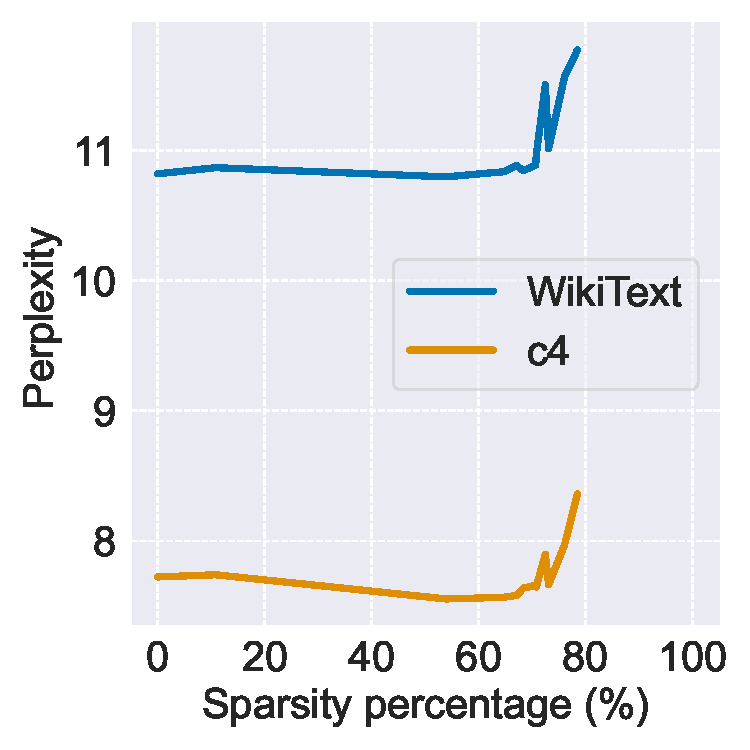
\includegraphics[width=0.248\textwidth]{figure/experiment/LLM.pdf}
  }
  \subfigure[Zero-Shot(Left). Five-Shot(Right)]{
    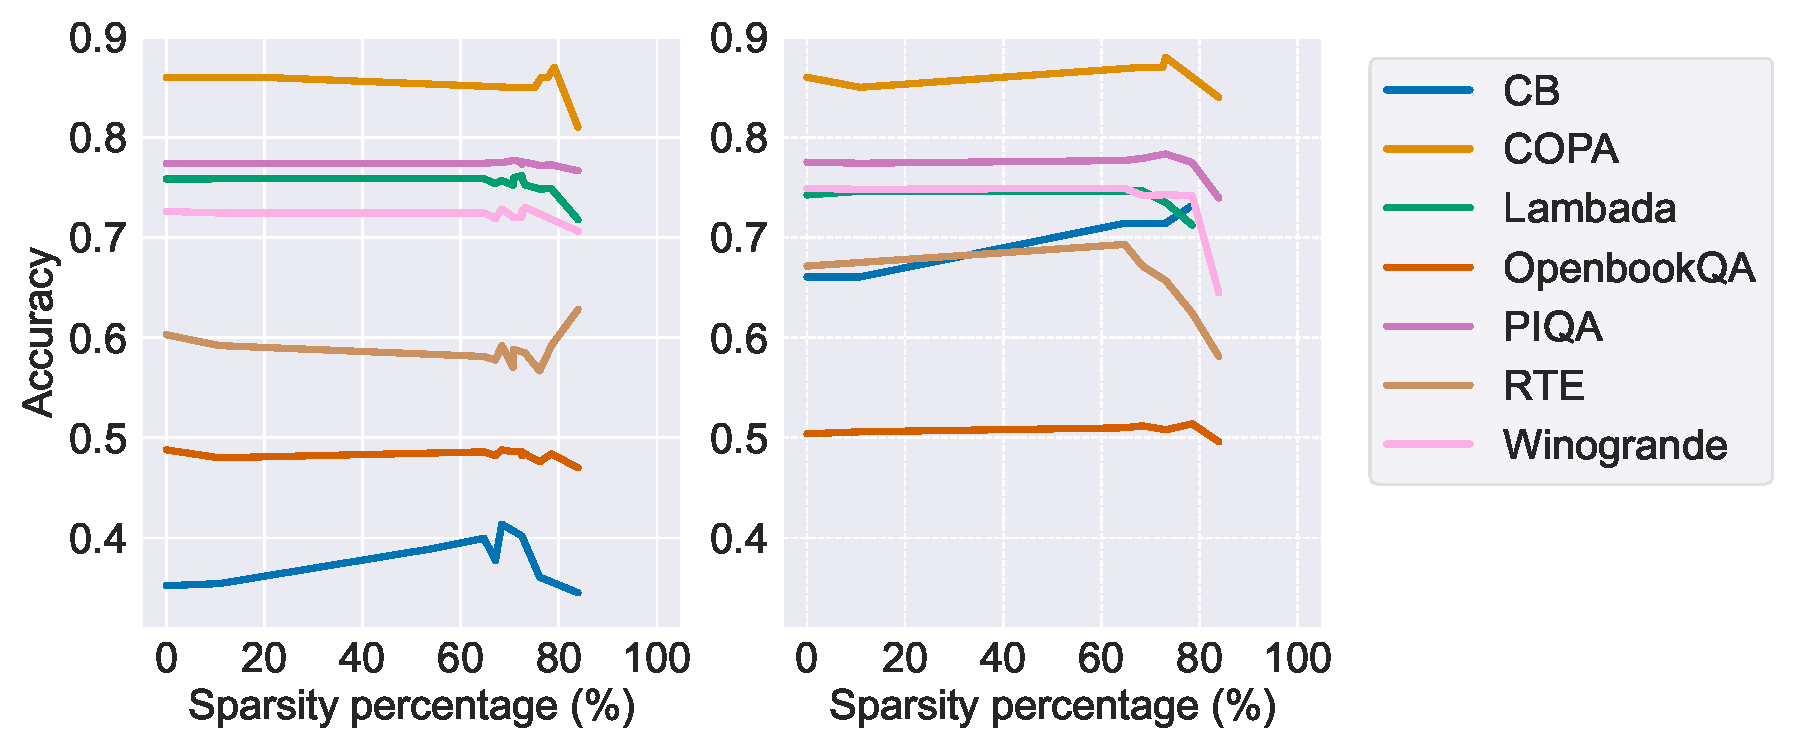
\includegraphics[width=0.61\textwidth]{figure/experiment/K_shot.pdf}
  }
  \vspace{-3mm}
  \caption{\textbf{ Accuracy Trend for \name{}-OPT-175B}. This figure shows the accuracy of \name{}-OPT-175B on language modeling datasets and downstream tasks when we set different sparsity at test time. In general, \name{}-OPT-175B incurs no accuracy drop until 75\% sparsity.\vspace{-1em}}
   \label{exp:kshot} 
\end{figure*}

\subsection{Hardware-efficient Implementation}
\label{sec:sparse_matmul}

We describe how \name{} is implemented in a hardware-efficient manner to realize the
theoretical speedup of contextual sparsity.
Taking into account hardware characteristics leads to over 2$\times$ speedup
compared to an optimized dense model, and 4$\times$ faster than a standard sparse
implementation.

\iffalse
Contextual sparsity requires us to multiply the feature vector $y$ with a sparse
subset of the weight matrices. For the attention QKV projection with projection
matrix $W^\mathrm{QKV}$ where we only
need the outputs of a few heads, we need to multiply
$W_\mathrm{qkv}[\mathrm{idx}, :] x_\mathrm{attn}$, where $\mathrm{idx}$ is a list of indices
corresponding to the heads whose outputs we need. The output projection of
the attention layer requires $W_\mathrm{out}[:, \mathrm{idx}] x_\mathrm{outproj}$. Sparsifying MLPs is similar.
\fi

We highlight some hardware characteristics of GPUs:
\begin{itemize}[itemsep=0.0pt,topsep=0pt,leftmargin=*]
  \item Small-batch generation is bottlenecked by GPU memory I/Os~\citep{nvidia2022nvidia, ivanov2021data, dao2022flashattention}. This is
  because of low arithmetic intensity. For each element loaded from GPU memory,
  only a small number of floating point operations are performed.
  \item GPUs are block-oriented devices: loading a single byte of memory takes
  the same time as loading a block of memory around that same
  address~\cite{harris2013access}. The block size is
  usually 128 bytes for NVIDIA GPUs~\citep{cook2012cuda}.
\end{itemize}
These characteristics present some challenges in implementing contextual
sparsity.
However, they can be addressed with classical techniques in GPU programming.
% \begin{itemize}[itemsep=0.1pt,topsep=0pt,leftmargin=*]

\textbf{Kernel fusion:} A standard implementation of sparse matrix-vector
  multiply (e.g., in PyTorch) that separately indexes a subset of the matrix
  $W^1_{S_M}$ before multiplying with input $y$ would incur 3$\times$ the
  amount of memory I/Os. Therefore, to avoid such overhead, we fuse the indexing and the multiplication step. Specifically, we load a subset of
  $W^1_{S_M}$ to memory, along with $y$, perform the multiply, then
  write down the result.
  This fused implementation (in Triton~\citep{tillet2019triton}) yields up to
  4$\times$ speedup compared to a standard PyTorch implementation (Appendix~\ref{sec:mlp_attn_benchmarks}).
  
\textbf{Memory coalescing:} In the dense implementation, the weight matrices of two linear layers in MLP are stored as $(W^1)^\top$ and $W^2$ so that no extra transpose operation is needed. They are conventionally stored in row-major format. In the sparse implementation, it allows us to load $(W^1_{S_M})^\top$ optimally (the second dimension is contiguous in memory). However, for cases where we need to load $(W^2_{S_M})$, this format significantly slows down memory loading, as indices in $S_M$ point to non-contiguous memory. We simply store these matrices in column-major format (i.e., store $(W^2)^\top$ in row-major format), then use the same fused kernel above. Similarly, in attention blocks, we store attention output projection $W^O$ column-major format.

These two techniques (kernel fusion and memory-coalescing) make \name{}
hardware-efficient, yielding up to 2$\times$ speedup end-to-end compared to the state-of-the-art FasterTransformer (Section~\ref{sec:main_result}).


% \begin{algorithm}[tb]
%    \caption{Deja Vu Model}
%    \label{alg}
% \begin{algorithmic}
%    \State{\bf Input:} data $x_i$, size $m$
% \end{algorithmic}
% \end{algorithm}




 


%%% Local Variables:
%%% mode: latex
%%% TeX-master: "main"
%%% End:
% is that In the Attention block, a number of attention heads are applied to a given input, and their outputs are concatenated.   Similar to MLP Block, a fast and accurate sparse prediction has to be identified without dense computation. 

% As we discussed in Section~\ref{sec:obs}, only a few heads perform heavy attending across tokens for a given input. 

% In the same Thus, we sparsify the attention block by selecting attention heads.


% In the Attention block, multiple attention heads are applied to a given input, and their outputs are concatenated. As we discussed in Section~\ref{sec:obs}, only a few heads perform heavy attending across tokens for a given input.  Thus, we sparsify the attention block by selecting attention heads.